\subsection{ITS Clusterization}
\label{recoFLP:ITS}

A simple clusterization algorithm was developed and tested within the
current \aliroot framework. It assumes row-wise arrival column-ordered
fired pixels data. Each input pixel with given \row, \col is tested
for possible attachment to clusters which are considered to be 
unfinished at the given moment. If it is not adjacent to any pixel in
one of such clusters, a new cluster candidate is created and
unfinished clusters with highest row number \row-2 are finalized. 
Currently the clusterization is performed for fired pixels shipped
within single readout frame only. Once the final readout architecture
will be selected, the algorithm may need to be modified to clusterize
across the neighbouring frames. The benchmarking with simulated data
shows the CPU time of 0.53 \ms per 1000 clusters (on single core of
Intel i7-2600 CPU @ 3.40 GHz processor) with full creation of clusters (
center of gravity and associated errors calculation). A benchmark of
alternative implementation \TBD{(S.~Chapeland, plain C, tested on
Intel Core i5-680  @ 3.60GHz)} shows 0.28 \ms per 1000 clusters. 
This translates to $\sim$110~Hz clusterization rate for minimum bias
\pbpb collisions at 50 kHz interaction rate, \TBD{assuming that the 
single-pixel noise can be tagged in the 
FE}. 
\TBD{This estimate does not take into account cluster data compression
and IO.}

The speed can be improved further, once the final format of the online input data will
be selected and we can profit from the "pre-clustering" done in the FE.

The following schema could be considered for the packaging of the
compressed cluster data of the single module, ordered in row then in
column directions (bending and non-bending directions; this ordering
is currently used in the reconstruction).

$m$ clusters of $n$-th module can be stored with Huffman compression in the format:
$\Delta modID_{n} \left[ (\Delta \row,\col, pattID)_{1} ... (\Delta \row,\col, pattID)_{m} \right]$, with
\row and \col referring on the pixel of cluster's center of gravity.
The $\Delta modID$ is the difference between the current and previously stored module identifiers,
similarly, the $\Delta$\row is the difference between the rows of current and previous cluster in the 
same module (0 for the first one). 
The pattern ID is a set of identifiers for cluster topologies like shown on Fig.~\ref{fig:clpatt}. 

\begin{figure}[h]
\centering
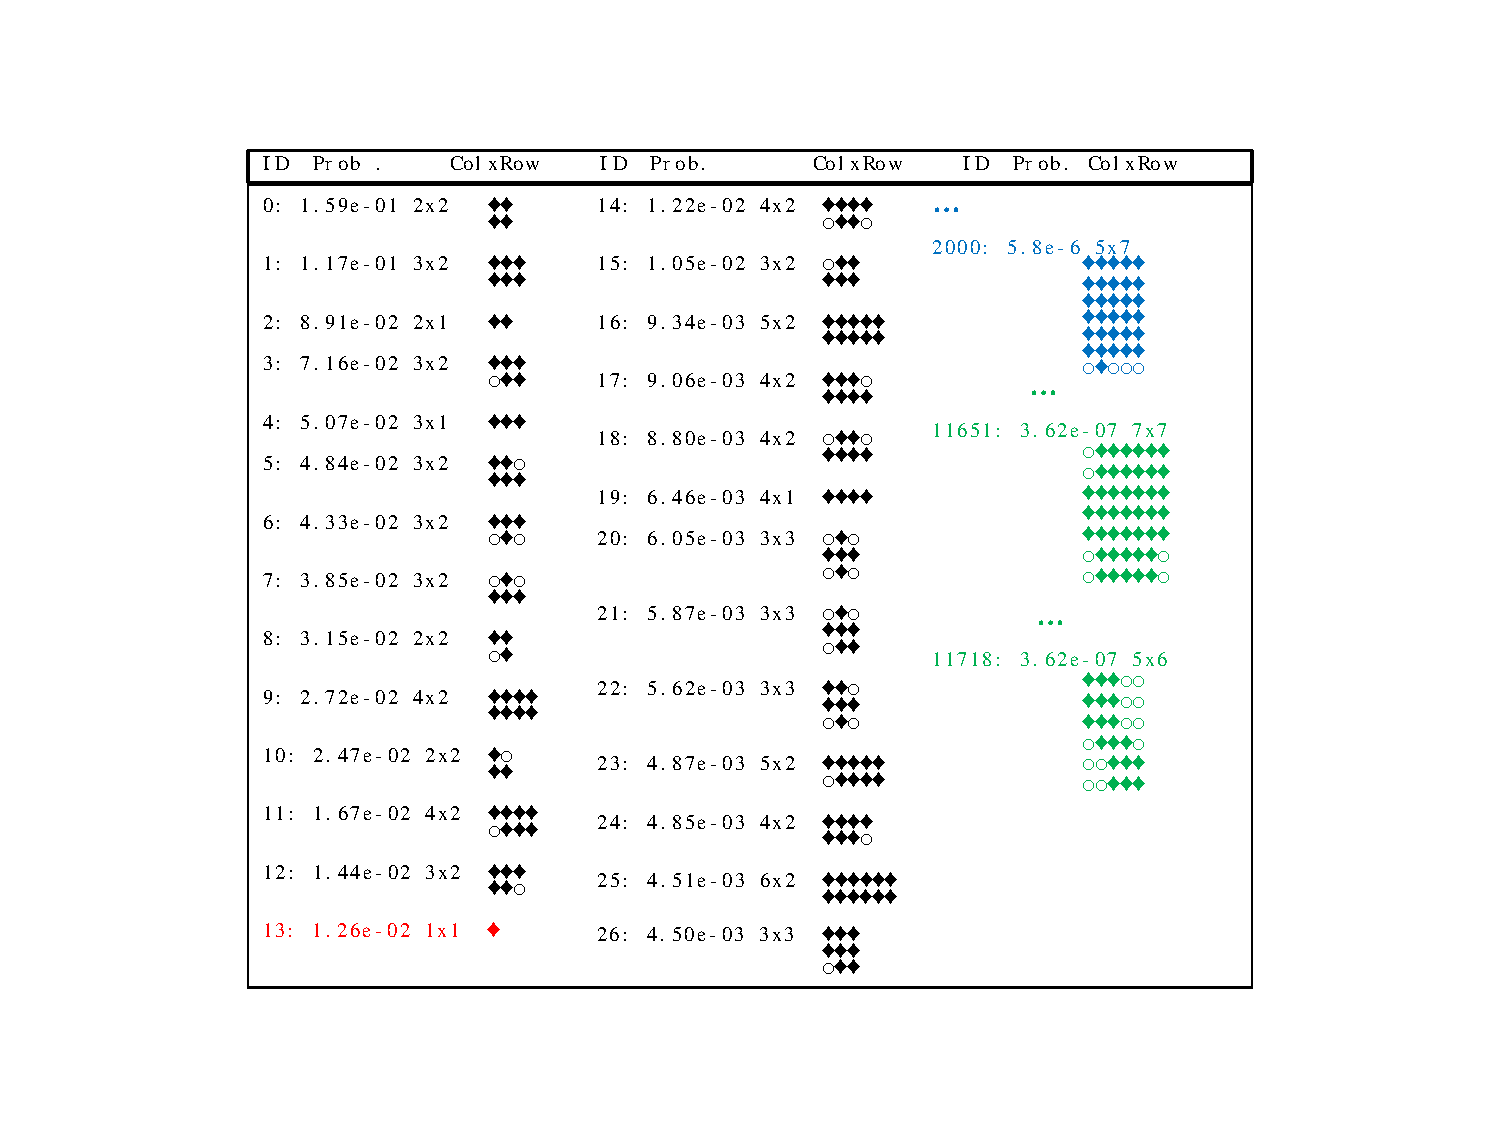
\includegraphics[trim=4.5cm 2cm 3.5cm 3cm , width=0.98\textwidth]{ITS/ClusPattDemo.pdf}
\caption{\label{fig:clpatt} 
Example of most and least frequent ITS clusters topologies. Column
"Prob" shows probability of given configuration while "Col$\times$Row"
is the dimension of smallest rectangle containing the pattern.}
\end{figure}

The probability
distribution of different patterns is shown on Fig.~\ref{fig:clpattHC}. We can assign dedicated ID to most probable
small cluster topologies and group a few patterns of rare large clusters with close topologies under the single ID.

\begin{figure}[h]
\centering
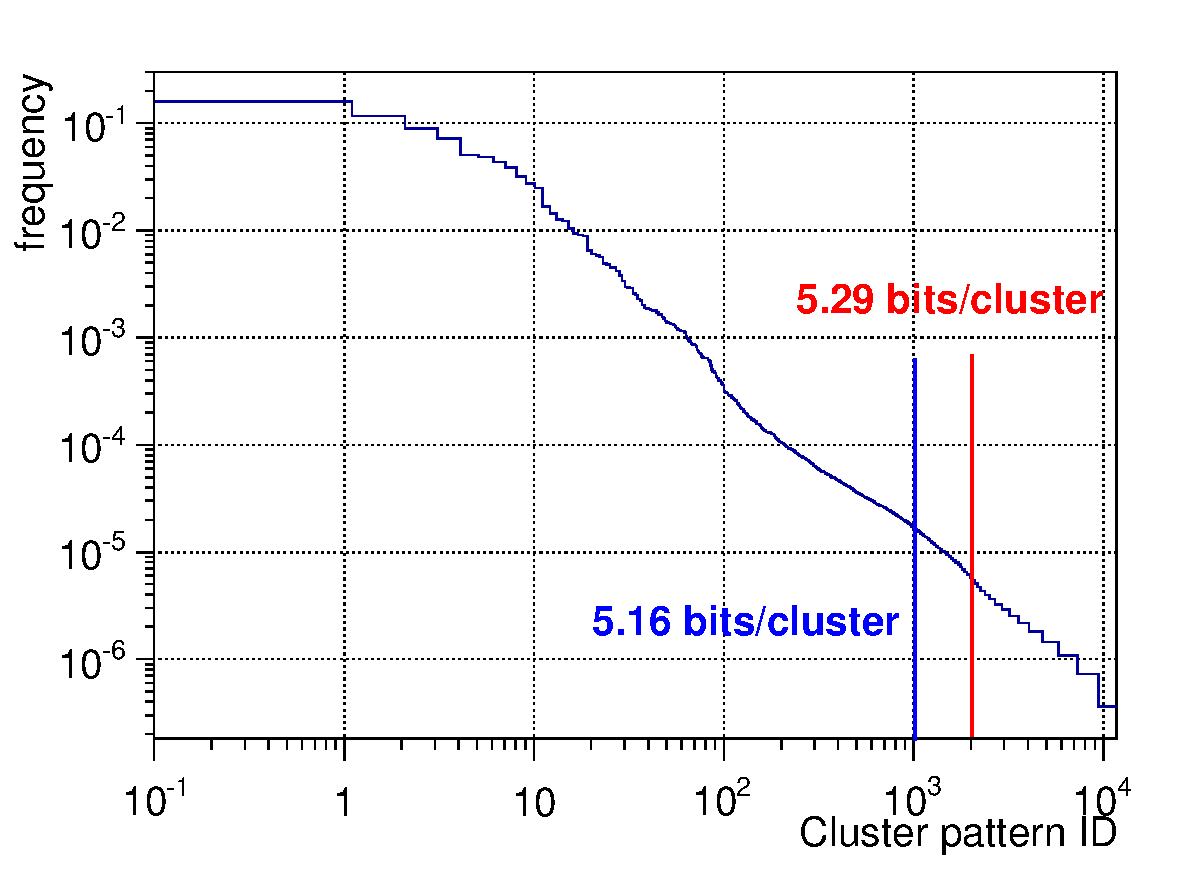
\includegraphics[width=0.9\textwidth]{ITS/ClusPattFreq.pdf}
\caption{\label{fig:clpattHC} 
Probability distribution of clusters with different ITS cluster topologies (see
Fig.~\ref{fig:clpatt}). The numbers refer to average (weighted) length
of the Huffman code for two choices of the number of pattern indices
to store.
Noisy pixels contribution is not accounted.
}
\end{figure}


If we define $\sim$2000 such IDs, using the Huffman coding we will need in average $\sim$5.3 bits per cluster if single-pixel
clusters are suppressed. In case we will need to keep the single-cluster pixels the average lenght of pattern ID record
will reduce to 1.8 bits for $10^{-5}$ noisy pixel probability.
Similarly, due to the ordering the probability distributions of $\Delta$\row and $\Delta modID$ are strongly non-uniform. 
Estimates show that we will need in average 1.2 bits per $\Delta modID$ and 7.3 bits per $\Delta$\row records in 
central \pbpb collision if single-pixel clusters are suppressed ($\Delta \row$ record will reduce to 
\TBD{<5 ?} if the single-pixel clusters are not suppressed). 
For peripheral collisions the compression factor for $\Delta \row$ deteriorates to \TBD{$\sim$10 and 7 bits
respectively}. The \col record will require $\sim$10.6 bits in average. 
Given that the $\Delta \row$ ($\Delta modId$) probability distributions strongly depend on the average number
of clusters in the module (readout frame) we will need to use different Huffman codes for the same type of record depending
on the multiplicity. 
In this way the storage clusters from single \pbpb collision will require $\sim$23 bits/cluster if the noise is rejected
and \TBD{$\sim$ 18} bits/cluster if the noise is kept. The corresponding preliminary estimate for the storage 
rate of \pbpb data at 50 kHz interaction rate is $\sim$5.3 GB/s discarding the single-pixel clusters while it would
stay $\sim$ 21 GB/s if the noise is not suppressed.
